\section{Non-functional Aspects}
\label{sec:comparativenonfunctional}

From a non-functional standpoint (even ignoring the performance aspect, discussed outside of this section, later on), GNS3 and CORE are relatively similar, but very different from Kathará, and therefore these aspects should be taken into account with the utmost attention.

\subsection{User Interface}
\label{subsec:comparativeui}

The differences in the user interface paradigm between GNS3 and CORE, on the one hand, and Kathará, on the other hand, were introduced in the presentation of Kathará in the examples of simulators (cf.~\ref{sec:exemulkathara}).
In particular, the fact that GNS3 and CORE's normal usage was thought out to be done through one or more instances of the GUI (more than one in case multiple users are concurrently and in a distributed fashion working on the same topology), while in Kathará a declarative, textual approach is necessary.

There isn't any GUI for operating Kathará in real-time.
The only graphical tool relatively compatible with that software package is a web-based app~\cite{netkitlabgen}, made for NetKit, which runs in the browser and allows to drag-and-drop elements into a canvas and parameterize, through web page forms, which interfaces are plugged to each, node startup IP addresses, etc., and then export a zipped directory with config files that Kathará, due to its backwards compatibility can import.
From our experience, this tool is very clumsy and incomplete.

In Kathará, users running similar experiments, maybe even the same ``lab'' (which is usually just a set of directories and text files), do it in their machine in total isolation.
Conversely, GNS3 introduces a conceptual client-server decoupling is exposed throughout the whole system.
Despite CORE's ``daemon'' and \gls{gui} being slightly different from the GNS3's server-client, practically it allows for the same flexibility~\cite{coredocs}.
This has an impact on how both are to be used and is caused, as will be seen in the next later in this chapter, by the difference in the weight both the projects (and their dependencies) themselves have and the resource consumption which, in GNS3, very easily creates the urge to balance the load.

% Figure fig:gns3-setup-wizard-servers
\begin{figure}
  \centering
  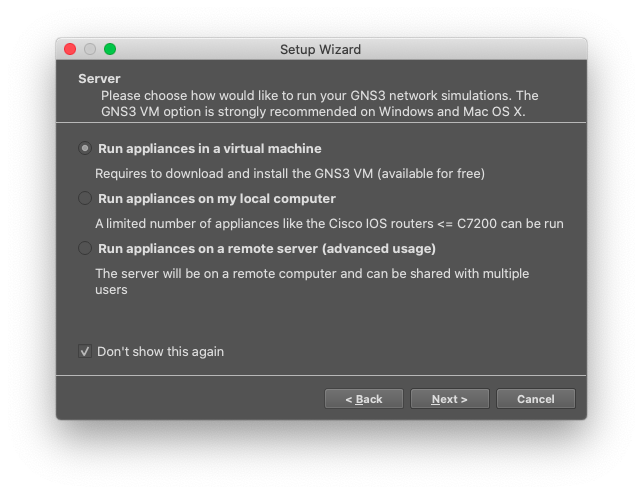
\includegraphics[width=0.8\textwidth]{comparative-gns3-setup-wizard-servers}
  \caption{The GNS3 setup wizard which shows on a fresh installation on by user's demand giving the options running GNS3 distributed}
  \label{fig:comparative-gns3-setup-wizard-servers}
\end{figure}


In GNS3, the project is running in the server, which, in many cases, is not the user's physical computer.
There is a notion of users connecting to the server (the open project), sharing resources and seeing the effects of actions done by action, which may require some protocols of coordination, e.g. given by the instructor.

\subsection{Portability and Sharability of Projects}
\label{subsec:comparativeportability}
In texts offering comparisons between network emulators and simulators~\cite{netkit-full,reproduciblenetexp}---in general, software based solutions to replace ``the real thing''---, this is an aspect that has to be taken into account.

On Kathará, if the default Docker images are used (or, in case they are customized, the extended images are published on Docker Hub, and they can always be) the labs are easily shareable and reproducible with the same behavior.

On GNS3, that is not the case.
The dependency
  \begin{enumerate*}[label=(\roman*), itemjoin={{, }}, itemjoin*={{, and }}]
  \item on the proprietary images for either Dynamips or IOSv
  \item in case of using IOSv, on a Linux host for QEMU/KVM support
  \item in case of using Docker nodes as end hosts, which the GNS3's computes can only interact with on Linux hosts, on that operating system
  \end{enumerate*}
as well as the possibility to have distributed labs across more than one server, literally separating the whole set of files needed to reproduce an experiment, and the heavy relying on randomly generated UUIDs, make this more difficult by orders of magnitude. % TODO add UUIDs to acronyms

% end of section comparativenonfunctional
